\chapter{数据模型初探}

数据本身只反映出现象,因此我们的目的不仅仅是搜集数据本身,而是通过数据发现背后的机理和规律——
不只是回答“怎么样”,更重要的是回答“为什么”。而发现数据中规律的重要方法就是数据模型。

\section{交通流模型}

以一条道路上的交通状态为例,我们可以用流量$q$、密度$k$、速度$v$三个指标来描述。
其中根据物理守恒定律很容易推导出$q=k\cdot v$,另一方面密度$k$和速度$v$之间的关系就不是那么直观了。对于这种未知的关系,我们可以用一个函数$v=f(k)$表示,$f$的数学定义就代表了速度和密度之间的关系,也是路段上交通状态变化的背后机理。

为了找出合适的函数$f$我们要从实际出发,首先通过各种手段实际观测道路上的流量、密度、速度。
直接从现实世界观测到的数据称为\emph{实测数据(empirical data)}%
\sidenote{empirical是一个哲学词汇,反义词是ideological。分别表示基于现实世界的的和基于意识形态的证据}
,大量数据如果以数字表格形式存在,我们很难理解。
因此第一步一般是将数据可视化,绘制成某种图形。

路段流密速数据一般可视化方法是以将每一条记录画作一个数据点,横坐标表示密度、纵坐标表示速度或流量。实测数据绘制后一般呈现出类似\cref{fig:empirical-qkv}的形态,从中马上可以看出一些规律。
例如从左图中速度和密度之间的关系,可以看出随着密度增加速度总体呈下降趋势;而且密度较小时速度下降不明显。从右图中流量和密度之间的关系,可以看出随着密度增加流量呈先上升后下降的趋势。

\begin{figure*}
    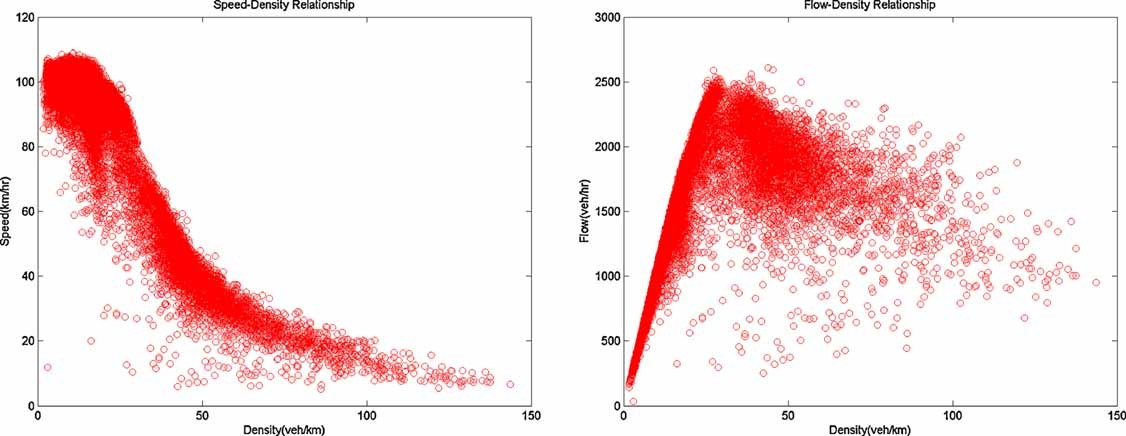
\includegraphics[width=\linewidth]{images/empirical-qkv.jpg}
    \caption{路段流量、密度、速度的典型实测数据}
    \label{fig:empirical-qkv}
\end{figure*}

由于我们已经知道$q=k\cdot v$,也就是说知道$k$,$v$就能计算出$q$,因此流量$q$对于我们来说是\emph{冗余数据(redundant data)},在后续分析中可以舍弃\sidenote{冗余数据并非没有价值,可以用于验证数据有效性。这里直接舍弃是为了简化讨论。}。此时我们面临的问题是,定义一个函数
\begin{equation}
    v=f(k)
\end{equation}
让该函数的图像与实测数据尽量符合,在数学上称为\emph{拟合问题}。

为了确定函数$f$的定义我们需要回答两个问题。第一个问题是函数的基本形态是什么?例如是直线、抛物线、还是指数曲线。这里我们假设$f$的图像是一条直线\sidenote{合理选取函数形式要综合考虑很多因素,没有标准答案,需要结合经验和对数据本身的理解。}
,也可以说$f$是\emph{线性函数}。
对于线性函数我们可以写出公式
\begin{equation}\label{eq:linear-kv}
    v = a\cdot k + b
\end{equation}
其中$a$和$b$是未知\emph{参数(parameter)}。
解析几何告诉我们$a$,$b$参数取值决定直线的形态,因此第二个个问题是$a$、$b$取值多少函数$f$与实测数据吻合\emph{最好}。

\section{线性回归}
为了确定\cref{eq:linear-kv}中的参数$a$、$b$我们需要用到一种叫做\emph{线性回归}的数学方法。
不过在正式介绍线性回归前,我们可以看一个简化的例子,方便理解为什么需要线性回归。

\subsection{线性方程}

假设我们实测的数据只有两组,即两个不同时刻的密度和速度,分别写作$p_1\coloneqq(k_1, v_1), p_2\coloneqq(k_2, v_2)$\sidenote{数学符号$\coloneqq$表示两边定义等价,读作“定义为”。}
,其中$p$代表数据点(point)。
此时图上只有两个数据点,函数$f$的图像是一条直线,显然当它同时穿过$p_1$、$p_2$时对数据的拟合最好。如何确定此时$a$、$b$的取值?

我们可以通过线性方程组来求解$a$、$b$。由于直线穿过两个数据点,以下两个方程必定成立:
\begin{equation}
    \left\{
    \begin{aligned}
        v_1 &= a\cdot k_1 + b \\
        v_2 &= a\cdot k_2 + b
    \end{aligned}\right.
\end{equation}
其中$a$、$b$是需要求解的未知数,可以用高斯消元法求解。
但这里我们先不求解,而是先把方程组写成线性代数的形式,方便后面的讨论。
首先将未知数写成单独分离,得到
\begin{equation}\label{eq:la-kv}
    \begin{bmatrix}
        v_1\\
        v_2
    \end{bmatrix}=
    \begin{bmatrix}
        k_1 & 1\\
        k_2 & 1
    \end{bmatrix}\cdot
    \begin{bmatrix}
        a\\
        b
    \end{bmatrix}
\end{equation}

可以看到方程由三项构成,我们分别规定用字母表示。其中左边是所有速度数据构成的向量%
\sidenote{注意区别$\Vv$和$v$,黑体字母$\Vv$表示向量,正常字母$v$表示标量。}
,写作$\Vv$;中间是一个权重(weight)矩阵,写作$\MW$;右边是由所有参数构成的矩阵,写作$\Vu$。此时\cref{eq:la-kv}进一步简化表示为
\begin{equation}
    \Vv=\MW\cdot\Vu
\end{equation}
如果权重矩阵$\MW$可逆,参数$a$、$b$可以通过以下公式计算
\begin{equation}\label{eq:la-eq}
    \begin{bmatrix}
        a\\
        b
    \end{bmatrix}=
    \Vu=\MW^{-1}\cdot\Vv
\end{equation}
而这里的权重矩阵$\MW=\big[
\begin{smallmatrix}
    k_1 & 1\\
    k_2 & 1
\end{smallmatrix}$\big]
是$2\times2$的正方形矩阵,一般来说可逆。

\subsection{最小二乘法}

现在我们重新做了一次测量,得到一组新的数据$p_3\coloneqq(k_3, v_3)$,此时问题的性质发生了变化。按照上一节的步骤我们得到线性方正组
\begin{equation}\label{eq:la-kv-3}
    \begin{bmatrix}
        v_1\\
        v_2\\
        v_3
    \end{bmatrix}=
    \begin{bmatrix}
        k_1 & 1\\
        k_2 & 1\\
        k_3 & 1
    \end{bmatrix}\cdot
    \begin{bmatrix}
        a\\
        b
    \end{bmatrix}
\end{equation}
但是此时权重矩阵的尺寸是$3\times2$,一般来说不可逆,无法求解$a$,$b$。
无法求解的原因是我们有两个未知量$a$、$b$,但是有三个约束条件分别来自数据$p_1$、$p_2$、$p_3$,这类问题在数学上称为\emph{过约束}问题。

线性回归是解决这类过约束问题的常见方法,能够在没有精确解的情况下求出最优近似解。
当线性方程组$\Vv=\MW\cdot\Vu$因为过约束无解时,方程两边同时乘以$\MW^{-1}$,将\cref{eq:la-eq}转化为以下\emph{最小二乘形式}
\begin{equation}\label{eq:least-square}
    \MW^{-1}\Vv=\MW^{-1}\MW\cdot\Vu
\end{equation}
此时方程是否有解由矩阵$\MW^{-1}\MW$是否可逆决定。
可以证明无论$\MW$是什么形状,$\MW^{-1}\MW$都是正方形矩阵,一般来说可逆。
为了与精确解区别,最佳近似解记作$\Vu^*$,可以通过以下公式计算
\begin{equation}
    \Vu^*=(\MW^{-1}\MW)^{-1}\MW^{-1}\Vv
\end{equation}

\begin{example}
    假设路段交通流的速度$v$和密度$k$之间的关系可以用线性函数$v=a\cdot k+b$描述。
    根据以下数据用线性回归方法确定参数$a$、$b$。
    \begin{center}
        \begin{tabular}{ccc}
            \toprule
            数据编号 & 速度(公里/小时) & 密度(辆/公里) \\
            \midrule
            1 & 80 & 10 \\
            2 & 50 & 100 \\
            3 & 20 & 150\\
            \bottomrule
        \end{tabular}
    \end{center}
\end{example}
\begin{solution}
    假设直线$v=a\cdot k+b$同时通过三个数据点,可以写出线性方程
    \begin{equation*}
        \MW\Vu=\Vv
    \end{equation*}
    其中
    \begin{equation*}
        \MW=
        \begin{bmatrix}
            10 & 1\\
            100 & 1\\
            150 & 1
        \end{bmatrix}\text{,}\quad
        \Vu=
        \begin{bmatrix}
            a\\
            b
        \end{bmatrix}\text{,}\quad
        \Vv=
        \begin{bmatrix}
            80\\
            50\\
            20
        \end{bmatrix}\text{。}
    \end{equation*}

    可以由于$\MW$矩阵的形状是$3\times2$方程无解,我们使用最小二乘法,在方程左右两侧同时乘以$\MW$的转置矩阵$\MW^T$,得到新的方程
    \begin{align*}
        \MW^T\MW\Vu&=\MW^T\Vv\\
        \intertext{代入数据得到}
        \begin{bmatrix}
            10 & 100 & 150\\
            1 & 1 & 1\\
        \end{bmatrix}
        \begin{bmatrix}
            10 & 1\\
            100 & 1\\
            150 & 1
        \end{bmatrix}
        \begin{bmatrix}
            a\\
            b
        \end{bmatrix}&=
        \begin{bmatrix}
            10 & 100 & 150\\
            1 & 1 & 1\\
        \end{bmatrix}
        \begin{bmatrix}
            80\\
            50\\
            20
        \end{bmatrix}\\
        \intertext{化简得到}
        \begin{bmatrix}
            32600 & 260\\
            260 & 3
        \end{bmatrix}
        \begin{bmatrix}
            a\\
            b
        \end{bmatrix}&=
        \begin{bmatrix}
            8800\\
            150\\
        \end{bmatrix}\\
        \intertext{解方程得到}
        \begin{bmatrix}
            a\\
            b
        \end{bmatrix}&=
        \begin{bmatrix}
            -\frac{63}{151}\\
            \frac{14010}{151}
        \end{bmatrix}
        \approx
        \begin{bmatrix}
            -0.417\\
            86.15
        \end{bmatrix}
    \end{align*}
\end{solution}


\section{线性回归原理}

\cref{eq:least-square}中我们直接给出了线性回归求解最佳近似解的方法,本节将解释为什么这个公式有效。要理解线性回归的原理,有代数和几何两个角度。其中代数角度的关键是残差平方和最小,几何角度的关键是向量空间的正交投影。以下将分别解释。

\subsection{残差平方和最小}
假定参数$a$,$b$为已知量,利用\cref{eq:linear-kv}可以根据密度$k$计算速度$v$。
此时一个密度对应两个速度,一个称为\emph{实测值}另一个称为\emph{预测值}。
例如密度$k_1$对应的实测值是$v_1$,预测值为了区别记作$\hat{v}_1=f(k_i)=ak_1+b$。
\nolinebreak\sidenote[][0cm]{$\hat{v}$读作“hat v”或者“帽子 v”}%
实测值和预测值之间的差别称为\emph{残差},记作$e_1=\hat{v}_1-v_1$。
理想情况下实测值与预测值吻合,残差$e_1=0$;如果做不到,越接近$0$越好。

\subsubsection{残差平方和}

当有多个数据点时,我们需要一个指标表示所有数据点预测值和估计值的总体吻合程度,常用的指标\emph{残差平方和(Sum of Squares Error)}定义为:
\begin{equation}\label{eq:sse}
    \text{SSE}=\sum_{i=1}^n {e_i}^2=\sum_{i=1}^n (v_i-f(k_i))^2
\end{equation}
其中$n$是数据点数量,$e_i$代表第$i$个数据点的残差。残差平方和并不是唯一的指标,首先介绍的原因是他有一些良好的性质,可以简化数学处理。
另一个常用的指标是\emph{残差绝对值之和}$\sum_{i=1}^{n}|e_i|$,虽然在数学处理上难度更高,但是在其他方面更有优势,会在后续章节介绍。

根据以上定义可以看出残差平方和$\text{SSE}$是参数$a$、$b$的函数,因为不同的$a$、$b$取值会影响预测值$\hat{v}$,进而影响到残差$e_i$,再而影响到残差平方和。需要特殊强调这个函数关系时残差平方和可以记作$\text{SSE}(a,b)$或者$\text{SSE}(\Vu)$,接下来我们推导它的公式。

根据\cref{eq:sse}的定义,我们可以把残差平方和写成向量\emph{点积}形式
\begin{equation}\label{eq:sse-vec}
    \begin{split}
        \text{SSE}&=\sum_{i=1}^n {e_i}^2=
        \begin{bmatrix}
            e_1 & e_2 &\cdots & e_n
        \end{bmatrix}
        \cdot
        \begin{bmatrix}
            e_1 \\
            e_2 \\
            \vdots\\
            e_n
        \end{bmatrix}\\
        &=\Ve^T\cdot\Ve
    \end{split}
\end{equation}
其中$\Ve=[\begin{smallmatrix}
    e_1 & e_2 & \cdots & e_n
\end{smallmatrix}]^T$是所有残差构成的列向量。
接下来我们写出残差向量$\Ve$的公式
\begin{equation}\label{eq:e-vec}
    \begin{split}
        \Ve=
        \begin{bmatrix}
            e_1 \\
            e_2 \\
            \vdots\\
            e_n
        \end{bmatrix}&=
        \begin{bmatrix}
            v_1 \\
            v_2 \\
            \vdots\\
            v_n
        \end{bmatrix}-
        a\cdot
        \begin{bmatrix}
            k_1 \\
            k_2 \\
            \vdots\\
            k_n
        \end{bmatrix}-
        b\cdot
        \begin{bmatrix}
            1 \\
            1 \\
            \vdots\\
            1
        \end{bmatrix}\\
        &=\Vv-a\Vk-b\vec{1}\\
        &=\Vv-\MW\Vu
    \end{split}
\end{equation}
其中$\Vv$是所有速度实测值的向量,$\MW$是权重矩阵,$\Vk$是所有密度数据的向量,$\vec{1}$是全$1$向量。

把\cref{eq:e-vec}带入\cref{eq:sse-vec},然后展开化简可以得到
\begin{align*}
    \text{SSE}(\Vu) &= \Ve^T\cdot\Ve\\
    &=(\Vv-\MW\Vu)^T(\Vv-\MW\Vu)\\
    &=\Vv^T\Vv+(\MW\Vu)^T\MW\Vu
    -\Vv^T\MW\Vu-(\MW\Vu)^T\Vv\\
    \intertext{使用向量点积的交换关系$\Va^T\Vb=\Vb^T\Va$得到}
    &=\Vv^T\Vv+(\MW\Vu)^T\MW\Vu
    -(\MW\Vu)^T\Vv-(\MW\Vu)^T\Vv\\
    \intertext{再使用矩阵转置的交换关系$(\MA\MB)^T=\MB^T\MA^T$,最终得到}
    \text{SSE}(\Vu) &=\Vu^T\MW^T\MW\Vu-2\Vu^T\MW^T\Vv-\Vv^T\Vv 
    \addtocounter{equation}{1}\tag{\theequation}
    \label{eq:sse-function}
\end{align*}

\subsubsection{残差平方和最小化}

通过推导我们写出了残差平方与参数之间公式$\text{SSE}(\Vu)$,接下来就是要找到特定的参数取值$\Vu=\Vu^*$,让$\text{SSE}(\Vu^*)$最小;
即$\text{SSE}(\Vu^*)\leq\text{SSE}(\Vu)\text{,}\forall\Vu$。
这是一个典型的\emph{最优化问题},可以记作
\sidenote{$\argmin$是“argumentum minimi”,最小化参数,的缩写;与之对应的是$\argmax$,“argumentum maximi”。}
\begin{equation}
    \Vu^*=\argmin \text{SSE}(\Vu)
\end{equation}

观察\cref{eq:sse-function},可以看到$\text{SSE}(\Vu)$的自变量$\Vu$虽然是向量,但是总体形式类似于一个抛物线函数$au^2-bu+c$。
利用微积分的知识,我们推测该函数存在最小值,且最小值处导数为$0$。由此我们列出方程
\begin{equation}
    \begin{split}
        \frac{\partial\text{SSE}}{\partial\Vu}(\Vu^*)&=\left[
        \frac{\Vu^T\MW^T\MW\Vu}{\partial\Vu}-
        \frac{2\Vu^T\MW^T\Vv}{\partial\Vu}-
        \frac{\Vv^T\Vv}{\partial\Vu}\right](\Vu^*)\\
        &=2\MW^T\MW\Vu^*-2\MW^T\Vv=0
    \end{split}
\end{equation}
整理最后两项我们得到\cref{eq:least-square}中的最小二乘形式,由此说明从代数角度理解,线性回归的意义是找出最优拟合参数,让残差平方和最小的。

\subsection{列向量空间正交投影}
\begin{figure}
    \def\svgwidth{\linewidth}
    %\fbox{\input{images/least-square-vector-space.pdf_tex}}
    \input{images/least-square-vector-space.pdf_tex}
\end{figure}
